\documentclass[notes]{beamer}
\usepackage[latin1]{inputenc}
\usepackage{tikz}
\usetikzlibrary{shapes.misc,calc,arrows,matrix}
\usepackage{verbatim}
\usepackage{amsthm}
\usepackage{stmaryrd} % To use double square brackets \llbracket, \rrbracket
\usetheme{Warsaw}
%\usetheme{default}

\title{Homogeneity is Independent from Randomness}
\author{Li Ling Ko}
\institute{University of Notre Dame}
\date{16 February, 2018}
\setbeamertemplate{footline}[frame number]
\setbeamertemplate{theorems}[numbered]

\newcommand{\TODO}[1]{\textcolor{red}{TODO: #1}}
\newtheorem{thm}{Theorem}
\newtheorem*{thm*}{Theorem}
\newtheorem*{main-thm*}{Main Theorem}
\newtheorem{coro}{Corollary}
\newtheorem*{coro*}{Corollary}
\newtheorem{pf}{Proof}
\newtheorem*{pf*}{Proof}
\newtheorem{define}{Definition}
\newtheorem*{define*}{Definition}
\newtheorem{claim}{Claim}
\newtheorem*{claim*}{Claim}
\newtheorem*{fact*}{Fact}
\newtheorem*{lemma*}{Lemma}
\newtheorem*{notation*}{Notation}
\newtheorem{observe}{Observe}
\newtheorem*{observe*}{Observe}
\newtheorem*{example*}{Example}
\newtheorem*{goal*}{Goal}

\begin{document}
\begin{frame}
  \titlepage
\end{frame}

\begin{frame}{Ramsey's Theorem asserts Homogeneity}
  \begin{define*}[$c$-homogeneous]
    Given $k$-coloring $c:[\omega]^n\rightarrow k$, a subset
    $A\subseteq\omega$ is \textbf{$c$-homogeneous} if every $n$-tuple over
    $A$ is given the same color by $c$.
  \end{define*}

  \vspace{0.5em}
  \begin{thm*}[Ramsey's]
    Fix $n,k\leq1$. \textbf{$\text{RT}_k^n$} is the statement that every
    $k$-coloring $c:[\omega]^n\rightarrow k$ has an infinite
    $c$-homogeneous set.\\
    \vspace{0.5em}
    \textbf{RT} is the statement $(\forall n)(\forall k)\; \text{RT}_k^n$.
  \end{thm*}
  \textbf{Proof sketch:} $\text{RT}_2^1$ holds since in any 2-coloring of
  $\omega$, one of the colors gives an infinite set. Induct on $n$ to get
  $\text{RT}_2^n$. Then inductively group colors together to get
  $\text{RT}_k^n$ from $\text{RT}_2^n$. $\square$

  \vspace{0.5em}
  \textbf{RT asserts homogeneity.}
\end{frame}

\begin{frame}{Lebesgue measure}
  \begin{define*}[Outer, inner measure]
    $\mu(\llbracket\sigma\rrbracket) =2^{-|\sigma|}$. The \textbf{outer
    measure} of $\mathcal{A}\subseteq2^\omega$ is
    \[\mu^*(\mathcal{A}):= \inf\left\{\sum_{n\in\omega}
    \mu(\llbracket\sigma_n\rrbracket): \mathcal{A}\subseteq
    \bigcup_{n\in\omega} \llbracket\sigma_n\rrbracket\right\}.\]
    Its \textbf{inner measure} is $\mu_*(\mathcal{A}):=
    1-\mu^*(\bar{\mathcal{A}})$.
  \end{define*}

  \begin{define*}[Lesbegue measure, null]
    $\mathcal{A}\subseteq2^\omega$ is \textbf{measurable} iff
    $\mu^*(\mathcal{A}) =\mu_*(\mathcal{A})$.  Then we say its
    \textbf{measure} is $\mu(\mathcal{A}) =\mu^*(\mathcal{A})
    =\mu_*(\mathcal{A})$. $\mathcal{A}$ is \textbf{null} iff
    $\mu(\mathcal{A})=0$.
  \end{define*}
  \begin{fact*}[Measurable]
    $\mathcal{A}\subseteq2^\omega$ is measurable iff it is
    $G_\delta$ (countable intersection of open sets) modulo a null. E.g.
    open sets, closed sets are measurable.
  \end{fact*}
\end{frame}

\begin{frame}{1-random}
  \begin{notation*}[Tree, real]
    The set of \textbf{reals} $A\in\omega^\omega$ contained in a
    \textbf{tree} $T\subseteq\omega^{<\omega}$ is denoted by $\llbracket
    T\rrbracket:= \{A\in\omega^\omega: (\exists n)\; [A\restriction n \in
    T]\}$.
  \end{notation*}

  \begin{define*}[Martin-Lof test of randomness]
    An effective enumeration of recursive trees $T_0,T_1,\ldots \subseteq
    2^{<\omega}$ is a \textbf{Martin-Lof test} if
    $\mu(\llbracket T_n\rrbracket) \leq 2^{-n}$ for all $n\in\omega$.\\
    \vspace{0.5em}
    A real $A\in2^\omega$ passes this test of randomness iff $A\not\in
    \bigcup_{n\in\omega} \llbracket T_n\rrbracket$.
  \end{define*}

  \begin{define*}[1-random]
    $A\in2^\omega$ is \textbf{1-random} if it passes every Martin-Lof test.
  \end{define*}
\end{frame}

\begin{frame}{Set of non 1-randoms is null}
  \begin{fact*}
    The set of reals that is not 1-random is null.
  \end{fact*}

  \vspace{2em}
  \textbf{Proof sketch:} There are only countably many Turing machines, so
  there can only be countably many Martin-Lof tests. The set of reals that
  fail a test is null since the trees in a test descend quickly. The union
  of a countable set of null sets is still null, thus the set of reals that
  fail some Martin-Lof test is null. $\square$
\end{frame}

\begin{frame}{WWKL asserts Randomness}
  \begin{thm*}[Weak Weak Konig's Lemma]
    If $T\subseteq 2^{<\omega}$ with positive measure i.e.
    \[\lim_n \frac{|\{\sigma\in T: |\sigma|=n\}|}{2^n} >0,\]
    it contains a real.
  \end{thm*}
  \begin{fact*}
    $T\subseteq2^{<\omega}$ has positive measure if and only if the set of
    reals with infinitely many initial segments contained in $T$ has
    positive measure.
  \end{fact*}

  \begin{coro*}
    If a binary tree has positive measure, it contains a 1-random.
  \end{coro*}

  \textbf{WWKL asserts randomness.}
\end{frame}

\begin{frame}{WWKL, WKL, KL}
  The reals of a WKL problem however, may all be non-randoms, because WKL
  includes also binary trees which are null:
  \begin{thm*}[Weak Konig's Lemma]
    Every binary tree with infinite nodes contains a real.
  \end{thm*}

  \vspace{2em}
  Konig's Lemma includes even trees that are not binary:
  \begin{thm*}[Konig's Lemma]
    Every finitely-branching tree with infinite nodes contains a real.
  \end{thm*}
\end{frame}

\begin{frame}{Homogeneity versus Randomness}
  A natural question to ask is which of the statements RT, KL, WKL, WWKL is
  stronger. Intuitively, WKL is stronger than WWKL, because a binary tree
  of positive measure has infinite nodes, so if all binary trees with
  infinite nodes have a real, then those with positive measure must
  have one too. A question that is harder to answer is:
  \newtheorem*{question*}{Question}
  \begin{question*}
    Which notion is stronger, homogeneity or randomness?
  \end{question*}
  If a given a real is homogeneous, does that say anything about how random
  it is? Likewise, if a given real is random, will it necessarily provide
  information on finding homogeneous reals?

  \vspace{0.5em}
  Since the notions of homogeneity and randomness are captured by RT and
  WWKL respectively, we are essentially asking which of RT and WWKL is
  stronger.
\end{frame}

\begin{frame}{Problem, Instance, Solution}
  \vspace{1em}
  \begin{define*}
    A mathematical \textbf{problem} is a collection of \textbf{instances},
    with a collection of \textbf{solutions} for each instance.
  \end{define*}

  \vspace{1em}
  \textbf{E.g. 1:} RT is a problem; its instances are the collections of
  colorings $c:[\omega]^n\rightarrow k$ for every $n,k\in\omega$, and the
  solutions of each $c$ are the class of $c$-homogeneous reals.

  \vspace{1em}
  \textbf{E.g. 2:} WWKL is a problem; its instances are the collections of
  binary trees with positive measure, and the solutions of each instance is
  the class of reals in the tree.
\end{frame}

\begin{frame}{Strongly Omnisciently Computably Reducible
($\leq_{\text{soc}}$)}
  \begin{define*}[Strongly Omnisciently Computably Reducible]
    Problem \textbf{P} is \textit{soc}-reducible to problem \textbf{Q}
    (written \textbf{P} $\leq_{\text{soc}}$ \textbf{Q}) if for every
    \textbf{P}-instance \textit{I}, there is a \textbf{Q}-instance
    \textit{J} such that every solution to \textit{J} computes a solution
    to \textit{I}.
  \end{define*}

  $\leq_{\text{soc}}$ successfully captures this expected relation:
  \begin{center}
    WWKL $\leq_{\text{soc}}$ WKL $\leq_{\text{soc}}$ KL.
  \end{center}

  \vspace{0.5em}
  \textbf{WWKL $\leq_{\text{soc}}$ WKL:} Given a binary tree with
  positive measure, this tree has infinite branches and is therefore an
  instance of WKL. The desired relation follows from definition of
  $\leq_{\text{soc}}$.

  \vspace{0.5em}
  \textbf{WKL $\leq_{\text{soc}}$ KL:} Given a binary tree with infinite
  branches, this tree is finitely-branching and therefore an instance of
  WKL. The desired relation follows from definition of $\leq_{\text{soc}}$.
\end{frame}

\begin{frame}{KL, RT $\leq_{\text{soc}}$ WKL}
  WKL is powerful under $\leq_{\text{soc}}$. Given any KL or RT
  instance, fix one of its solutions, and choose the WKL instance whose only
  real codes that solution as an real in $2^\omega$. By definition of
  $\leq_{\text{soc}}$, the given instance reduces to this WKL instance.

  \vspace{1em}
  For example, given a KL instance, fix one of its solutions
  $f:\omega\rightarrow\omega$, code this solution as a real in $2^\omega$
  in a recoverable manner.

  \vspace{1em}
  For instance, if $f$ is $2,9,3,\ldots$, we can code $f$ as the real
  $110$ $1111111110$ $1110\ldots$.

  \vspace{1em}
  Similarly, any solution of an RT instance can be seen as an infinite
  subset of $\omega$. Its characteristic function will be a real in
  $2^\omega$.
\end{frame}

\begin{frame}{Homogeneity ``independent from'' Randomness}
  Dependencies under $\leq_{\text{soc}}$
  \vspace{2em}

  \begin{center}
    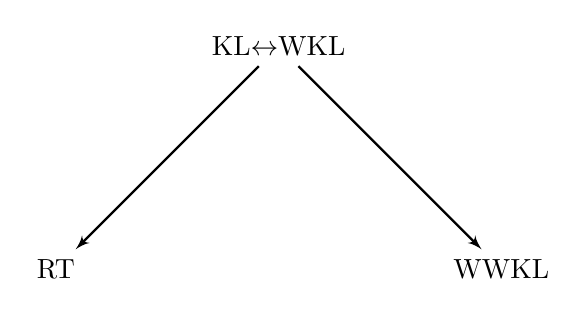
\begin{tikzpicture}[node distance=4cm,auto,thick,>=latex']
      \node (KL) {KL$\leftrightarrow$WKL};
      \node (WWKL) [below right of=KL] {WWKL};
      \node (RT) [below left of=KL] {RT};
      \draw[->] (KL) -- (RT);
      \draw[->] (KL) -- (WWKL);
      %\draw [->,red] (RT) -- coordinate (m) (WWKL);
      %\draw[shift={(m)},red](-0.1,-0.1)--(0.1,+0.1);
    \end{tikzpicture}
  \end{center}
\end{frame}

\begin{frame}{Bi-Hyperimmune sets}
  \begin{define}
    $X\subseteq\omega$ is \textbf{hyperimmune} if there is no recursive
    function $f$ such that $f(n)>p_X(n)$ for every $n\in\omega$.
  \end{define}

  \begin{define}
    $X$ is \textbf{bi-hyperimmune} if both $X$ and $\bar{X}$ are hyperimmune.
  \end{define}

  \begin{thm}
    Bi-hyperimmune sets exist.
  \end{thm}

  \vspace{0.5em}
  \textbf{Pf:} Enumerate recursive functions $f_0,f_1,\ldots$. At stage
  $s$, let $i$ be the number of elements in $X$ and $\bar{X}$ that has been
  defined so far. Put enough elements into $\bar{X}$ till the $(i+1)$-th
  element of $X$ exceeds $f_s(i+1)$. Repeat with roles of $X$ and $\bar{X}$
  reversed. $\blacksquare$
\end{frame}

\begin{frame}{Class of sets computing subsets of hyperimmune is null}
  \begin{thm}
    \label{thm:bihyper-null}
    Given a hyperimmune set $X$, the class of sets that can compute an
    infinite subset of $X$ is null.
  \end{thm}

  \vspace{1em}
  \textbf{Pf:} The idea is, if the class is not null, there are enough
  reals computing subsets of $X$ that one can effectively get them to
  ``vote'' for when new elements of $X$ have appeared, contradicting
  hyperimmunity of $X$.

  \vspace{1em}
  Given arbitrary Turing functional $\Phi$, let
  \[\mathcal{B} :=\{A: \Phi^A \subseteq X\; \text{infinite}\}.\]
  It is enough to show $\mathcal{B}$ is null since the union of countably
  many null sets is null.
\end{frame}

\begin{frame}{Class of sets computing subsets of hyperimmune is null}
  Assume by contradiction $\mu(\mathcal{B})=4m>0$.\\
  Tightly approximate $\mathcal{B}$ by open cover
  $\mathcal{U}'\supseteq\mathcal{B}$ so
  $\mu(\mathcal{U}'-\mathcal{B})<m$.\\
  Tightly approximate $\mathcal{U}'$ by $\mathcal{U} :=[\sigma_0] \cup
  \ldots\cup[\sigma_n] \subseteq\mathcal{U}'$ so
  $\mu(\mathcal{U}'-\mathcal{U}) <m$.\\
  Then $\mathcal{U}$ approximates $\mathcal{B}$ tightly enough that
  \begin{align*}
    \mu(\{A\in\mathcal{U}: \Phi^A \subseteq X\; \text{infinite}\}) &>2m,\\
    \mu(\{A\in\mathcal{U}: \Phi^A \not\subseteq X\; \text{infinite}\}) &<2m.
  \end{align*}

  To effectively dominate the $k$-th element of $X$, enumerate the nodes in
  $\mathcal{U}$. Wait till a measure of $2m$ of them find $k$-elements. By
  tight approximation, such nodes exist, and one of them must be an initial
  segment of a real that computes an infinite subset of $X$. Thus the
  $k$-th element of $X$ must be below the largest element found by all
  these nodes. $\blacksquare$
\end{frame}

\begin{frame}{$\text{RT}_2^1$ $\nleq_{\text{soc}}$ WWKL}
  \begin{thm}
    $\text{RT}_2^1$ $\nleq_{\text{soc}}$ WWKL.
  \end{thm}

  \vspace{1em}
  \textbf{Pf:} Let $c:\omega\rightarrow\{0,1\}$ be a 2-coloring of the
  graph of a fixed bi-hyperimmune $X$, that is,
  \[c(n)=0 \Leftrightarrow n\in X.\]
  
  From hyperimmunity of $X$ and $\bar{X}$, the class of sets computing an
  infinite subset of $X$ or of $\bar{X}$ is null. Equivalently, the class
  of $c$-homogeneous sets is null. Therefore given arbitrary tree
  $T\subseteq\omega^{<\omega}$ of positive measure, some real must fail to
  compute any $c$-homogeneous set. $\blacksquare$
\end{frame}

\begin{frame}{Homogeneity is not weaker than Randomness}
  \begin{coro}[RT $\nleq_{\text{soc}}$ WWKL]
    $\text{RT}_2^1$ $\nleq_{\text{soc}}$ WWKL. $\blacksquare$
  \end{coro}
  \begin{coro}[WKL $\nleq_{\text{soc}}$ WWKL]
    RT $\leq_{soc}$ WKL, RT $\nleq_{\text{soc}}$ WWKL. $\blacksquare$
  \end{coro}

  \vspace{1em}
  \begin{center}
    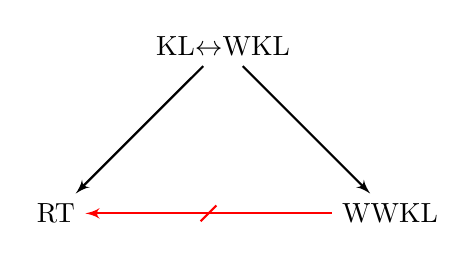
\begin{tikzpicture}[node distance=3cm,auto,thick,>=latex']
      \node (KL) {KL$\leftrightarrow$WKL};
      \node (WWKL) [below right of=KL] {WWKL};
      \node (RT) [below left of=KL] {RT};
      \draw[->] (KL) -- (RT);
      \draw[->] (KL) -- (WWKL);
      \draw [<-,red] (RT) -- coordinate (m) (WWKL);
      \draw[shift={(m)},red](-0.1,-0.1)--(0.1,+0.1);
    \end{tikzpicture}
  \end{center}
\end{frame}

\begin{frame}{Homogeneity does not imply Randomness}
  \begin{center}
    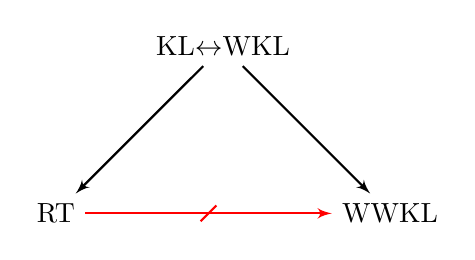
\begin{tikzpicture}[node distance=3cm,auto,thick,>=latex']
      \node (KL) {KL$\leftrightarrow$WKL};
      \node (WWKL) [below right of=KL] {WWKL};
      \node (RT) [below left of=KL] {RT};
      \draw[->] (KL) -- (RT);
      \draw[->] (KL) -- (WWKL);
      \draw [->,red] (RT) -- coordinate (m) (WWKL);
      \draw[shift={(m)},red](-0.1,-0.1)--(0.1,+0.1);
    \end{tikzpicture}
  \end{center}

  \begin{define*}
    $\mathcal{A}\subseteq\omega^\omega$ is $\Sigma_1^1$ iff there is a
    computable predicate $R(f,g)$ such that
    \[\mathcal{A} =\{f\in\omega^\omega: (\exists g)\; [R(f,g)]\}.\]
  \end{define*}

  \begin{main-thm*}[Monin, Patey, 2016]
    $\mathcal{C}\subseteq\omega^\omega$ compact, contains no
    $\Sigma_1^1$-subset ($\neq\emptyset$). Then there exists infinite set
    $X$ whose subsets cannot compute any real in $\mathcal{C}$.
  \end{main-thm*}
\end{frame}

\begin{frame}{Every $\Sigma_1^1$-set of $2^\omega$ contains an $O$-recursive}
  \begin{fact}
    \label{fact:sigma-contains-O-recursive}
    Every $\Sigma_1^1$-set of $2^\omega$ contains an $O$-recursive.
  \end{fact}

  \textbf{Pf (sketch):} Given a nonempty $\Sigma_1^1$-set
  \[\mathcal{A} =\{f\in2^\omega: (\exists g)\; R(f,g)\},\]
  observe that for a given $\sigma,\tau\in 2^{<\omega}$, the set \[\{f\succ
  \sigma: (\exists g\succ\tau)\; R(f,g)\}\] is also $\Sigma^1_1$. Since
  every $\Sigma^1_1$-set is $O$-recursive, $O$ can enumerate the $\langle
  \sigma,\tau \rangle$ pairs for which the above set is nonempty.
  Arbitrarily long pairs exist since $\mathcal{A}$ is nonempty. Thus, $O$
  can iteratively construct a real $f=\bigcup_{s\in\omega} \sigma_s$ in
  $\mathcal{A}$, and $g=\bigcup_{s\in\omega} \tau_s$ witnessing
  $f\in\mathcal{A}$. $\square$
\end{frame}

\begin{frame}{Tree of positive measure with no $\Sigma_1^1$-subset}
  \begin{thm}
    There is a tree $T\subset2^{<\omega}$ such that $[T]\subset
    2^\omega$ is compact, has positive measure, and contains no
    $\Sigma_1^1$-subset ($\neq\emptyset$).
  \end{thm}

  \vspace{2em}
  \textbf{Pf:} Let $T\subset2^{<\omega}$ be a set of 1-randoms
  relativized to Kleene's $O$. Then $[T]\subset 2^\omega$ has positive
  measure, and is closed and therefore compact. Also, $T$ has no nonempty
  $\Sigma_1^1$-subset from the previous fact that every $\Sigma^1_1$-set
  contains an $O$-recursive. $\blacksquare$
\end{frame}

\begin{frame}{Homogeneity does not imply Randomness}
  \begin{theorem}
    WWKL $\nleq_{\text{soc}}$ RT.
  \end{theorem}

  \vspace{1em}
  \textbf{Pf:} Let $T\subset2^{<\omega}$ be the tree from the previous
  theorem, and let $c:[\omega]^n\rightarrow k$ be an arbitrary
  $k$-coloring. Recall:
  \begin{main-thm*}
    $\mathcal{C}\subseteq\omega^\omega$ compact, contains no
    $\Sigma_1^1$-subset ($\neq\emptyset$). Then there exists infinite set
    $X$ whose subsets cannot compute any real in $\mathcal{C}$.
  \end{main-thm*}

  \vspace{1em}
  The main theorem gives an infinite $X$ whose subsets cannot compute any
  real in $[T]$. Let $Y\subseteq X$ be an infinite subset of $X$ that is
  $c$-homogeneous. Then $Y$ is a $c$-homogeneous set that cannot compute
  any real in $[T]$. $\blacksquare$
\end{frame}

\begin{frame}{Homogeneity ``independent from'' Randomness}
  \begin{coro}[WKL $\nleq_{\text{soc}}$ RT]
    WWKL $\leq_{soc}$ WKL, WWKL $\nleq_{\text{soc}}$ RT. $\blacksquare$
  \end{coro}

  \vspace{2em}
  \begin{center}
    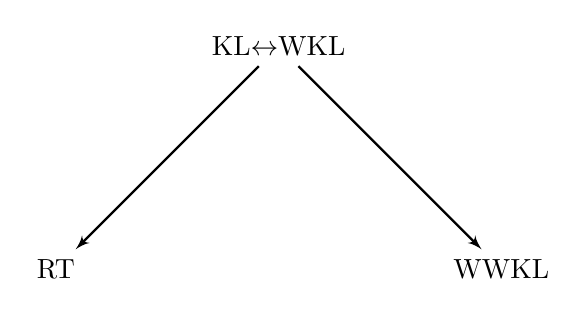
\begin{tikzpicture}[node distance=4cm,auto,thick,>=latex']
      \node (KL) {KL$\leftrightarrow$WKL};
      \node (WWKL) [below right of=KL] {WWKL};
      \node (RT) [below left of=KL] {RT};
      \draw[->] (KL) -- (RT);
      \draw[->] (KL) -- (WWKL);
      %\draw [<-,red] (RT) -- coordinate (m) (WWKL);
      %\draw[shift={(m)},red](-0.1,-0.1)--(0.1,+0.1);
    \end{tikzpicture}
  \end{center}
\end{frame}

\begin{frame}{$\Sigma_1^{1}$-immunity basis theorem (fixed predicate)}
  \begin{lemma*}[$\Sigma_1^{1}$-immunity basis, fixed predicate]
    $\mathcal{C}$ compact, contains no $\Sigma_1^{1}$-set
    ($\neq\emptyset$). Fix $\Sigma_1^{1}$-predicate $P(X,Y)$,
    $\Sigma_1^{1}$-set $\mathcal{D}_0\neq\emptyset$. Then
    $\mathcal{D}_0$ has a $\Sigma_1^{1}$-subset
    $\mathcal{D}\neq\emptyset$ such that for every $X\in\mathcal{D}$,
    $\mathcal{C}$ does not contain the $\Sigma_1^{1,X}$-set
    $\{Y:P(X,Y)\}$.
  \end{lemma*}

  \vspace{1em}
  \textbf{Pf:} \underline{Case 1}: For every $X\in\mathcal{D}_0$,
  $\{Y:P(X,Y)\}\subseteq\mathcal{C}$. Then $\bigcup_{X\in\mathcal{D}_0}
  \{Y:P(X,Y)\}$ will be a $\Sigma_1^{1}$-subset of $\mathcal{C}$,
  $\Rightarrow\Leftarrow$.

  \vspace{1em}
  \underline{Case 2}: For some $X_0\in\mathcal{D}_0$, $\{Y:P(X_0,Y)\}$
  contains a real $Y_0$ outside $\mathcal{C}$. By compactness of
  $\mathcal{C}$, $Y_0$ has an initial segment $\sigma$ outside
  $\mathcal{C}$. This $\Sigma_1^{1}$-subset of $\mathcal{D}_0$ works:
  \[\mathcal{D}:= \{X\in\mathcal{D}_0: (\exists Y\succ\sigma)\; P(X,Y)\}.\;
  \blacksquare\]
\end{frame}

\begin{frame}{Gandy-Harrington topology is Baire}
  \begin{thm*}[Gandy-Harrington topology is Baire]
    The topology on $\omega^\omega$ where open sets are generated by the
    $\Sigma_1^{1}$-sets is known as the Gandy-Harrington topology. This
    topology is Baire, i.e. the countable union of dense open sets is
    dense.
  \end{thm*}

  \vspace{1em}
  \textbf{Pf:} Given dense open sets $\mathcal{D}_0,\mathcal{D}_1,\ldots$
  and open set $\mathcal{U}=\{f:(\exists g)\; R(f,g)\}$, iteratively
  construct $f\in\bigcap_{n\in\omega}\mathcal{D}_n$ and $g$ witnessing
  $f\in\mathcal{U}$:
  
  \vspace{1em}
  At stage $n$, $[f\restriction n]\cap\mathcal{U} \neq\emptyset$, witnessed
  by an extension of $g\restriction n$. Now the class of reals in
  $[f\restriction n]$ that lie in $\mathcal{U}$ by a witness extending
  $g\restriction n$ is an open set, so it intersects
  $\mathcal{D}_0\cap\ldots\cap\mathcal{D}_{n+1}$. Thus one can choose
  $f\restriction (n+1) \succ f\restriction n$ in this intersection, and
  $g\restriction (n+1) \succ g\restriction n$ witnessing $[f\restriction
  (n+1)]\cap\mathcal{U} \neq\emptyset$. $\blacksquare$
\end{frame}

\begin{frame}{$\Sigma_1^{1,Z}$-immunity basis theorem}
  \begin{thm*}[$\Sigma_1^{1}$-immunity basis]
    $\mathcal{C}$ compact, contains no $\Sigma_1^{1}$-set
    ($\neq\emptyset$). Fix $\Sigma_1^{1}$-set
    $\mathcal{D}\neq\emptyset$. Then $\mathcal{D}$ contains some $X$ such
    that $\mathcal{C}$ contains no $\Sigma_1^{1,X}$-set ($\neq\emptyset$).
  \end{thm*}
  \textbf{Pf:} For each $\Sigma_1^{1}$-predicate $P$, let $\mathcal{U}_P$
  be the union of all the $\Sigma_1^{1}$-sets where every $X$ in the set
  gives a real outside $\mathcal{C}$ via $P$. From previous lemma,
  $\mathcal{U}_P$ is dense under Gandy-Harrington topology. This topology
  is Baire, so $\bigcap_P\mathcal{U}_P$ is non-empty. Any
  $X\in\bigcap_P\mathcal{U}_P$ works. $\blacksquare$

  \vspace{0.5em}
  \begin{coro*}[$\Sigma_1^{1,Z}$-immunity basis]
    $\mathcal{C}$ compact, contains no $\Sigma_1^{1,Z}$-set
    ($\neq\emptyset$). Fix $\Sigma_1^{1,Z}$-set
    $\mathcal{D}\neq\emptyset$. Then $\mathcal{D}$ contains some $X$ such
    that $\mathcal{C}$ contains no $\Sigma_1^{1,X}$-set ($\neq\emptyset$).
  \end{coro*}
  \textbf{Pf:} Directly relativize every step in the proof.
  $\blacksquare$
\end{frame}

\begin{frame}{Galvin-Prikry}
  \begin{fact*}[Galvin-Prikry]
    Given infinite set $Z\subseteq\omega$, node $\sigma\in\omega^{<\omega}$,
    and Turing functional $\Gamma:2^\omega\rightarrow\omega$, there exists
    an infinite subset $X\subseteq Z$ where one of these holds:\\

    \vspace{1em}
    \textbf{Positive-solution:} All subsets of $X$ compute (via $\Gamma$)
    $\sigma$ \\
    \textbf{Negative-solution:} All subsets of $X$ do not compute (via
    $\Gamma$) $\sigma$
  \end{fact*}

  \vspace{1em}
  \textbf{Proof sketch:} The class of subsets of $Z$ that
  compute $\sigma$ can be coded to form an open set in $2^\omega$. Being
  open provides enough ``structure'' for regions of homogeneity to exist.
  $\square$
\end{frame}

\begin{frame}{Galvin-Prikry}
  \begin{fact*}[Galvin-Prikry]
    Given infinite set $Z\subseteq\omega$, node $\sigma\in\omega^{<\omega}$,
    and Turing functional $\Phi:2^\omega\rightarrow \omega^{<\omega}$,
    there exists an infinite subset $X\subseteq Z$ where one of these
    holds:\\

    \vspace{1em}
    \textbf{Positive-solution:} All inf. subsets of $X$ compute (via
    $\Phi$) $\sigma$ \\
    \textbf{Negative-solution:} All inf. subsets of $X$ don't compute (via
    $\Phi$) $\sigma$
  \end{fact*}

  \vspace{1em}
  \textbf{Pf (sketch):} The class of subsets of $Z$ that compute (via
  $\Phi$) $\sigma$ can be coded to form an open set in $2^\omega$, by the
  finite use principle. Being open provides enough ``structure'' for
  regions of homogeneity to exist. $\square$
\end{frame}

\begin{frame}{Set whose subsets cannot compute reals in $\mathcal{C}$}
  \newtheorem*{main-lemma*}{Main Lemma}
  \begin{main-lemma*}[Monin, Patey, 2016]
    \begin{align*}
      \text{Given } &\begin{cases}
        \mathcal{C}\subseteq\omega^\omega \text{ compact, contains
        no nonempty } \Sigma^{1,Z}_1\text{-set},\\
        \text{Turing functional } \Phi:2^{\omega}\rightarrow
        \omega^{<\omega},
      \end{cases}
    \end{align*}
    $Z$ contains an infinite subset $X\subseteq Z$ whose subsets cannot
    compute (via $\Phi$) any real in $\mathcal{C}$.
  \end{main-lemma*}

  \vspace{3em}
  \textbf{Pf:} \textbf{Case 0:} There is a node outside
  $\mathcal{C}$ with a positive GP-solution $X$. This $X$ works since
  all its subsets compute (via $\Phi$) a node outside $\mathcal{C}$.
\end{frame}

\begin{frame}{Set whose subsets cannot compute reals in $\mathcal{C}$
(cont.)}
  \textbf{Case 1:} Every node outside $\mathcal{C}$ has only negative
  GP-solutions, and $\mathcal{C}$ has arbitrarily long nodes with
  positive GP-solutions. By compactness of $\mathcal{C}$, this set of
  nodes contains a real in $\mathcal{C}$. Then
  \begin{align*}
    \emptyset\neq\; &\{f:(\forall \sigma\prec f)\; [\sigma\; \text{has
    positive GP-solutions}]\}\\
    \subseteq\; &\{f:(\forall \sigma\prec f) (\exists \text{ inf }
    X\subseteq Z) (\forall \text{ fin } X_0\subset X) (\exists \text{ fin }
    X_1\subset X)\\ &\;\;\;\;\;\;[X_0 \prec X_1 \wedge
    \Phi^{X_1}(\sigma)\downarrow]\}
  \end{align*}
  is a nonempty $\Sigma_1^{1,Z}$-set contained
  in $\mathcal{C}$, $\Rightarrow\Leftarrow$.
\end{frame}

\begin{frame}{Set whose subsets cannot compute reals in $\mathcal{C}$
(cont.)}
  \textbf{Case 2:} For some $n$, every node $\sigma_0,\ldots,\sigma_m$ in
  $\mathcal{C}$ of length $n$ has only negative GP-solutions. Iterate GP
  across them to get decreasing subsets of negative solutions
  \[Z=X_0 \supseteq X_1 \supseteq \ldots\supseteq X_m=X,\]
  where $X_{i+1}\subseteq X_i$ is a negative GP-solution under inputs
  $X_i$ and $\sigma_i$. $X_{i+1}$ exists since GP gives only negative
  solutions for each $\sigma_i$ under $Z$, giving also only negative
  solutions under $X_i\subseteq Z$.

  \vspace{0.5em}
  Take $X=X_m$. Then every subset of $X$ cannot compute (via $\Phi$) any
  node in $\mathcal{C}$ of length exceeding $n$, and in particular,
  cannot compute any real in $\mathcal{C}$. $\blacksquare$

  \vspace{0.5em}
  \textbf{Note:} Each $X_{i+1}$ is picked from the $\Sigma^{1,X_i}_1$-set
  \begin{align*}
    &\{Y:Y\subseteq X_i \text{ inf } \wedge Y \text{ is a
    negative GP-solution for } \sigma_i]\}\\
    =\;&\{Y:Y\subseteq X_i \text{ inf } \wedge (\forall \text{ fin }
    Y_0\subset Y)\; [\Phi^{Y_0}(\sigma_i)\uparrow]\}.
  \end{align*}
\end{frame}

\begin{frame}{Set whose subsets cannot compute reals in $\mathcal{C}$
(relativized)}
  \begin{main-lemma*}[\textcolor{red}{Relativized}]
    \begin{align*}
      \text{Given } &\begin{cases}
        \mathcal{C}\subseteq\omega^\omega \text{ compact, contains
        no nonempty } \Sigma^{1,Z}_1\text{-set},\\
        \text{Turing functional } \Phi:2^{\omega}\rightarrow
        \omega^{<\omega},
      \end{cases}
    \end{align*}
    $Z$ contains an infinite subset $X\subseteq Z$ whose subsets cannot
    compute (via $\Phi$) any real in $\mathcal{C}$.\\
    \vspace{0.5em}
    \textcolor{red}{Furthermore, we can choose $X$ such that $\mathcal{C}$
    also contains no nonempty $\Sigma_1^{1,X}$-subset.}
  \end{main-lemma*}

  \textbf{Pf:} In the proof of the non-relativized lemma, $Z=X_0
  \supseteq \ldots\supseteq X_m=X$, and $X_{i+1}$ is picked from a
  $\Sigma^{1,X_i}_1$-set. The immunity-basis theorem asserts
  that every such set contains some $X_{i+1}$ such that $\mathcal{C}$
  contains no $\Sigma_1^{1,X_{i+1}}$-set, if $\mathcal{C}$ contains no
  $\Sigma^{1,X_i}_1$-subset. Iterate this theorem across $X_i$'s.
  $\blacksquare$
\end{frame}

\begin{frame}{Preserving initial segment}
  \begin{main-lemma*}[Relativized, \textcolor{red}{Segment-preserving}]
    \begin{align*}
      \text{Given } &\begin{cases}
        \mathcal{C}\subseteq\omega^\omega \text{ compact, contains
        no nonempty } \Sigma^{1,Z}_1\text{-set},\\
        \text{Turing functional } \Phi:2^{\omega}\rightarrow
        \omega^{<\omega},
      \end{cases}
    \end{align*}
    $Z$ contains an infinite subset $X\subseteq Z$ whose subsets cannot
    compute (via $\Phi$) any real in $\mathcal{C}$.\\
    \vspace{0.5em}
    Furthermore, we can choose $X$ such that $\mathcal{C}$ also contains no
    nonempty $\Sigma_1^{1,X}$-subset.\\
    \vspace{0.5em}
    \textcolor{red}{Finally, given $s\in\omega$, $X$ can be chosen to
    preserve $Z\restriction s$.}
  \end{main-lemma*}

  \vspace{1em}
  \textbf{Pf:} The idea is to iterate the relativized lemma across all
  subsets of $Z\restriction s$. Iteration is possible after relativization.
\end{frame}

\begin{frame}{Preserving initial segment (cont.)}
  List the subsets of $Z\restriction s$ as $d_0,\ldots,d_n$. Iterate the
  relativized lemma across them to get decreasing subsets
  \[Z=X_0 \supseteq X_1 \supseteq X_2 \supseteq\ldots \supseteq X_n.\]
  At stage $i$, apply lemma with inputs $X_i$, and $\Phi_i$ defined by
  \[\Phi_i(Y) =\Phi(Y\cup d_i),\]

  giving $X_{i+1}\subseteq X_i$ whose subsets cannot compute (via
  $\Phi_i$) reals of $\mathcal{C}$, and where $\mathcal{C}$ contains no
  nonempty $\Sigma_1^{1,X_i}$-set.

  \vspace{1em}
  Choose $X=X_n\cup Z\restriction s$. Since $X$ almost equals $X_n$ and
  $\mathcal{C}$ contains no $\Sigma_1^{1,X_n}$-set, $\mathcal{C}$ also
  contains no $\Sigma_1^{1,X}$-set. Let $Y\subseteq X$ with $Y\restriction
  i=d_i$. Stage $i$ ensured that the subsets of $Y$ compute no real in
  $\mathcal{C}$ via $\Phi_i$. Since $Y\supset d_i$, the same is ensured via
  $\Phi$. $\blacksquare$
\end{frame}

\begin{frame}{Set whose subsets cannot compute reals in $\mathcal{C}$}
  \begin{main-thm*}[Monin, Patey, 2016]
    $\mathcal{C}\subseteq\omega^\omega$ compact, contains no
    $\Sigma_1^1$-subset ($\neq\emptyset$). Then there exists infinite set
    $X$ whose subsets cannot compute any real in $\mathcal{C}$.
  \end{main-thm*}

  \vspace{1em}
  \textbf{Pf:} The main lemma worked for fixed functional $\Phi$. Iterate
  the lemma across all functionals $\Phi_0,\Phi_1,\ldots$ to construct
  decreasing subsets of $X$'s
  \[\omega= X_0\supseteq X_1\supseteq\ldots,\]
  where at stage $s$, the lemma is applied with inputs $X_s$ and
  $\Phi_s$, and $X_{s+1}$ preserves the first $s$-elements of $X_s$. Take
  $X=\bigcap_{s\in\omega}X_s$; this $X$ is infinite from
  segment-preservation. $\blacksquare$
\end{frame}

\end{document}
